\section{Analysis method and results}

\subsection{$\alpha_{T}$ selection}

The single-lepton analysis cut-flow starts with the requirement of exactly one ``good'' lepton (electron or muon), with $p_{T} > 5$ GeV, in the event. The jet cuts has been driven by the all-hadronic N-jet analysis and constist in the requirement of at least two jets with $p_{T}>30 \textrm{GeV}$ and $|\eta|<3$. The second jet must have $p_{T}>100 \textrm{GeV}$. An $H_{T}$ cut at 350 GeV is applied in addition, in order to select events with significant amount of hadronic-jet activity relevant to the SUSY environment. The final step in the selection consists of the requirement that the variable $\alpha_{T}$ should be above $0.55$. This cut is expected to supress (almost) all of the QCD N-jets (including $b\bar{b} + \textrm{jets}$) events, as explained earlier.

Figures ~\ref{fig:dists1} and ~\ref{fig:dists2} display the distributions of basic kinematic observables that are utilized in the analysis, for all the SM backgrounds and the SUSY signal (LM0 and LM1), after the standard selection but the $\alpha_{T}$ cut. Such observables, besides the $\alpha_{T}$ itself, are basically the recoil missing transverse energy, $MH_{T}$, defined as the vectorial sum of the energies of all jets plus the lepton in the event:
\begin{eqnarray}
MH_{T}= - \sum_{i = 1,..,N} p_{T}^{i , \textrm{jet}} + p_{T}^{\ell}
\end{eqnarray} 
and the scalar sum of the energies of all jets plus the lepton, $H_{T}$. All of these observables provide a discriminating power of the SUSY signal over the SM expectations, to some extent. As will be proven in the next sections, the $\alpha_{T}$ variable is the dominant cutting variable in terms of robustness and control over QCD jet mismeasurements.

\begin{figure}[h!]
\begin{minipage}[b]{0.5\linewidth}
\centering
{\label{fig:aT}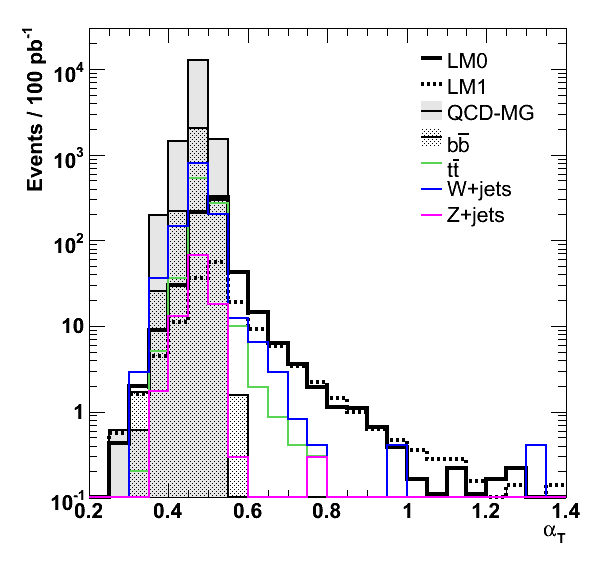
\includegraphics[scale=0.38]{./plots/aT-AllSignals.png}} 
\end{minipage}
\begin{minipage}[b]{0.5\linewidth}
\centering
{\label{fig:mht}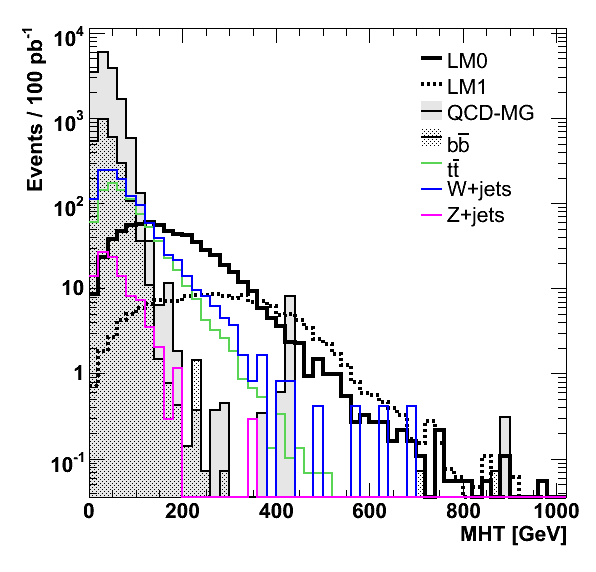
\includegraphics[scale=0.38]{./plots/MHT-AllSignals.png}} 
\end{minipage}
%\subfigure[The $\alpha_{T}$ distribution after all cuts but $\alpha_{T}$.]{\label{fig:aT}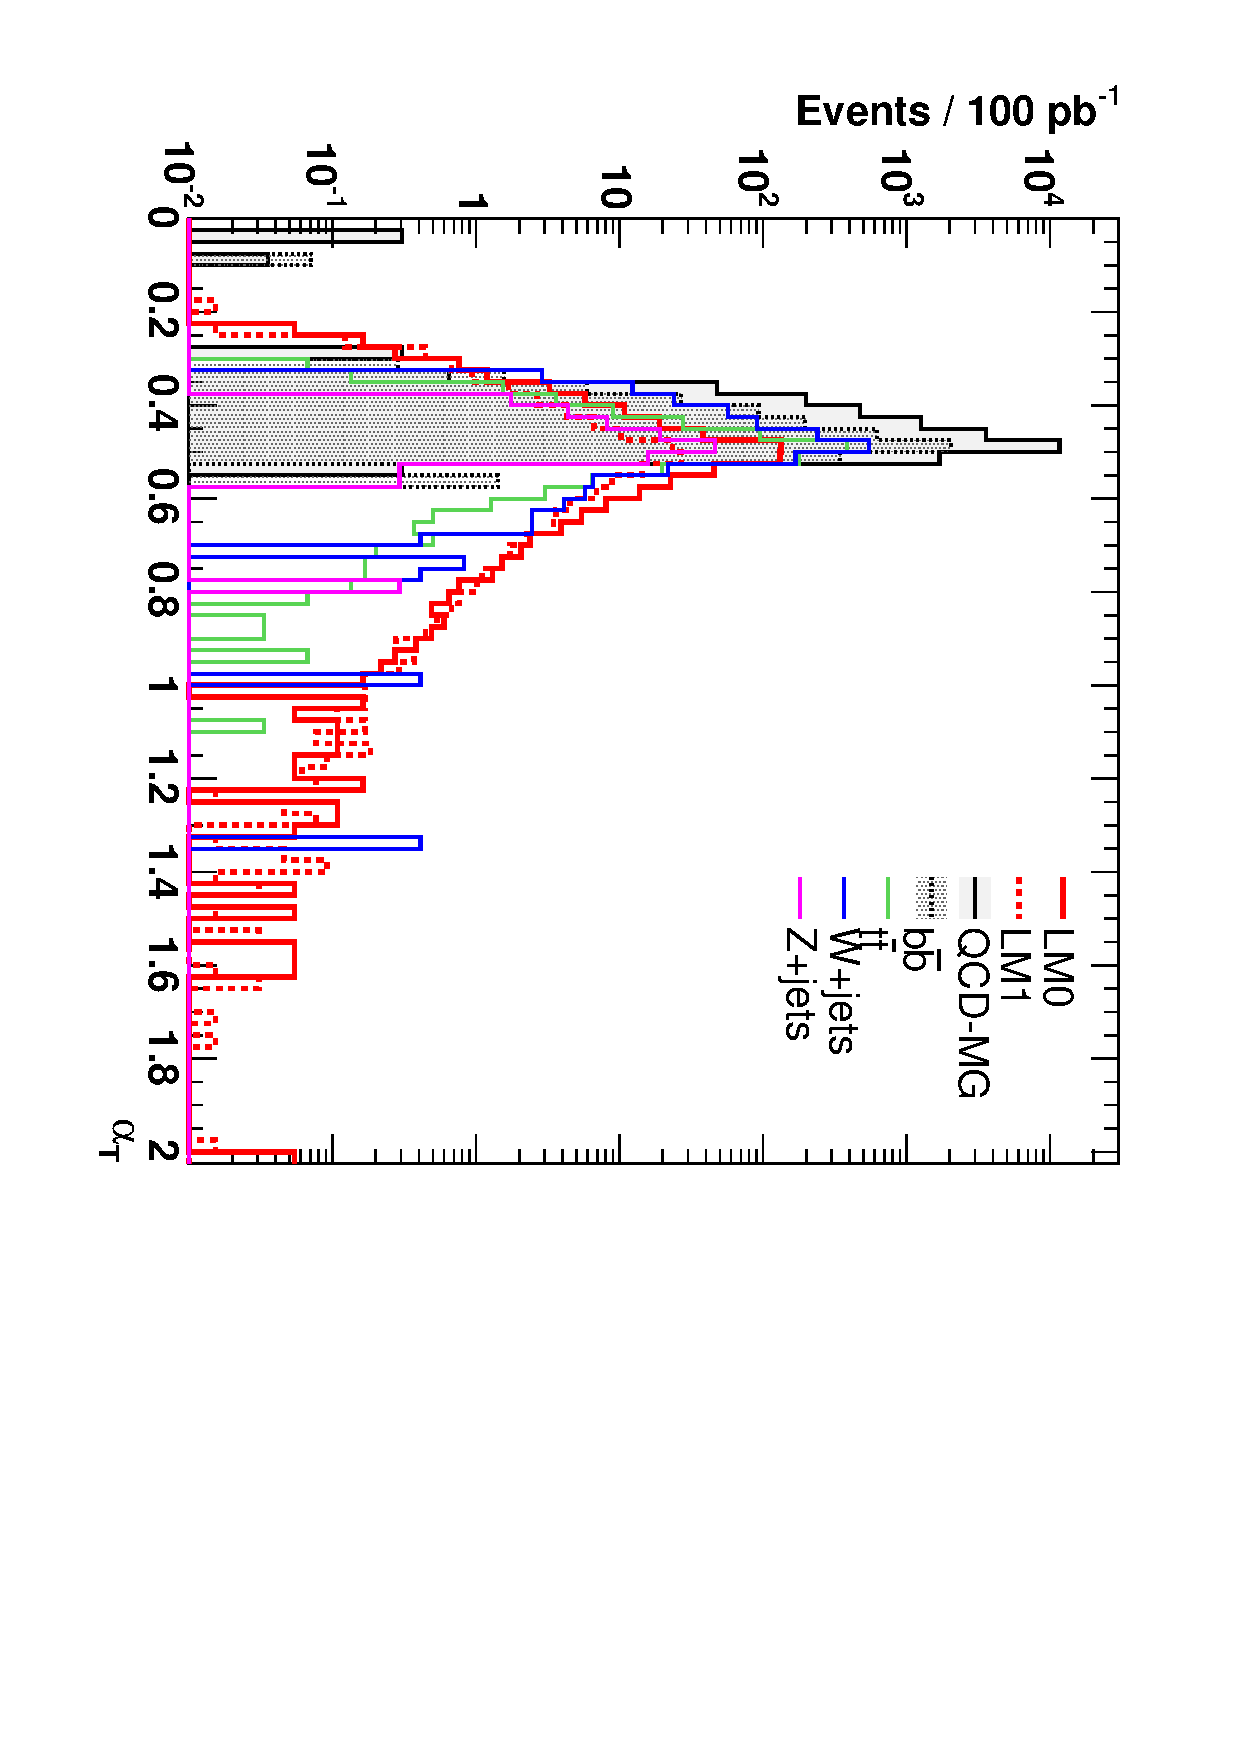
\includegraphics[scale=0.4, angle=90]{./plots/aT-NT7-SigAndBkg-AfterHTcut}} 
%\subfigure[The $\textrm{MH}_{\textrm{T}}$ distribution after all cuts but $\alpha_{T}$.]{\label{fig:mht}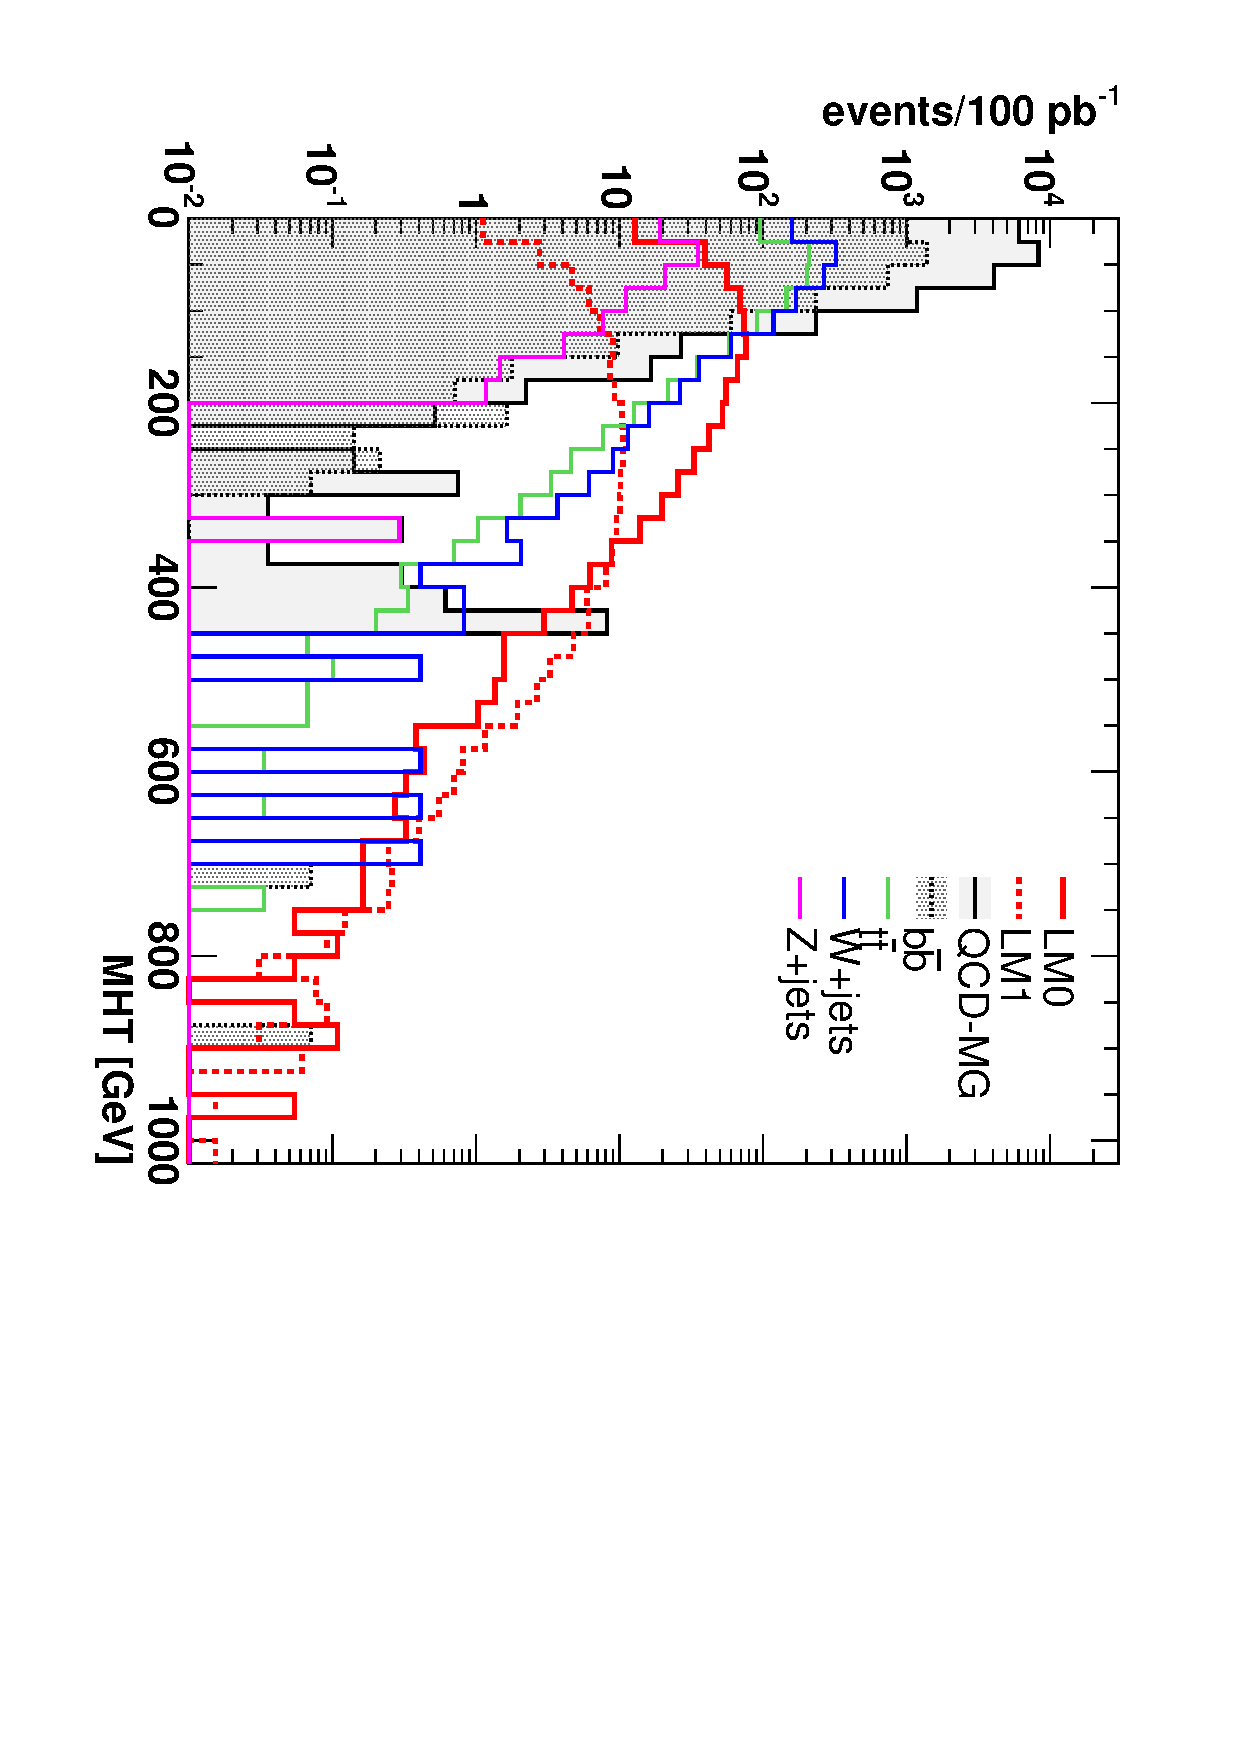
\includegraphics[scale=0.4,angle=90]{./plots/MHT-NT7-SigAndBkg-AfterHTcut}} 
\caption{\textit{The $\alpha_{T}$ (a) and $MH_{T}$ (b) distributions for the LM0 and LM1 SUSY signal and all the SM backgrounds superimposed, for an integrated luminosity of $100 \textrm{pb}^{-1}$.} }
\label{fig:dists1}
\end{figure}
\begin{figure}[h!]
\begin{minipage}[b]{0.5\linewidth}
\centering
{\label{fig:mhtovht}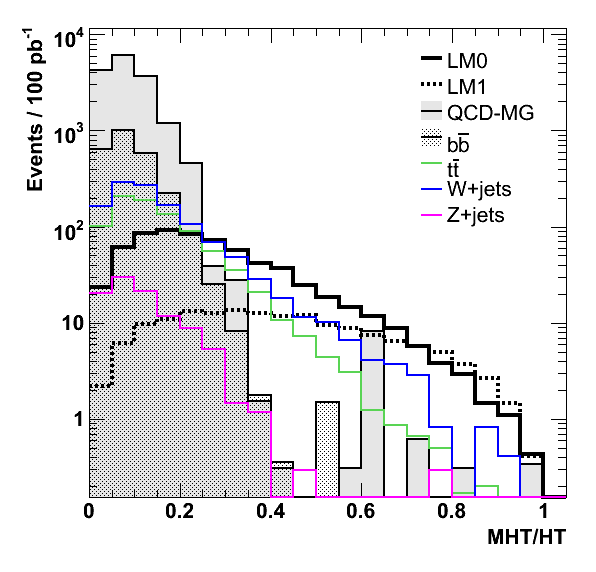
\includegraphics[scale=0.38]{./plots/MHTovHT-AllSignals.png}} 
\end{minipage}
\begin{minipage}[b]{0.5\linewidth}
\centering
{\label{fig:ht}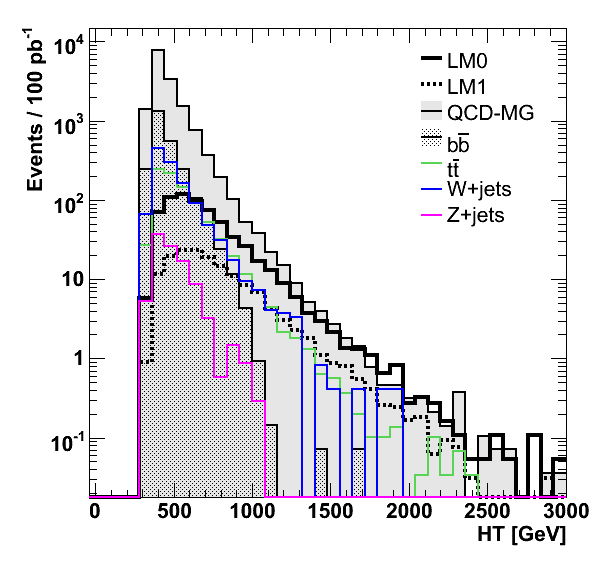
\includegraphics[scale=0.38]{./plots/HT-AllSignals.png}} 
\end{minipage}
\caption{\textit{The $MH_{T}/H_{T}$ (a) and $H_{T}$ (b) distributions for the LM0 and LM1 SUSY signal and all the SM backgrounds superimposed, for an integrated luminosity of $100 \textrm{pb}^{-1}$.} }
\vspace{5mm}
\label{fig:dists2}
\end{figure}


\subsection{Comparison with RA4}

For the sake of completeness, a comparison of the event yields between the $\alpha_{T}$ cut-flow and the RA4 selection, normalized for $100 \textrm{pb}^{-1}$ of integrated luminosity, is presented next.

The RA4 selection follows a more traditional cut-flow involving a cut in the missing transverse energy. From Monte Carlo (MC) studies, it has been shown that the missing energy variable provides a fairly good separation between the SUSY signal events, in R-parity conserving models, and most of the SM background processes ($W/Z + \textrm{jets}, t\bar{t} + \textrm{jets}$ and QCD ). Although, originally the MET cut in RA4 is rather loose (set to $100$ GeV)\footnote{A loose cut in the missing energy at $100$ GeV has been set to RA4, as the most suitable cut for the LM0 events separation, but also to allow a significant event yield in order to allow further cuts for background estimation purposes (ABCD method etc).}, we alternatively try to tighten the cut at $180$ GeV, which seems to be an optimal cut value for most of the LMx SUSY points, for the purpose of comparison with the $\alpha_{T}$ approach.

The event pre-selection for the two analysis paths ($\alpha_{T}$ versus RA4), show rather different in the two approaches:
\begin{description}
\item[$a_{T}$ approach:] i) Exactly one muon or one electron with $p_{T}>5$ GeV, while vetoing a second different-flavor lepton. Both electron and muon objects are required to satisfy the customly proposed isolation. ii) Veto on events with: a second lepton not passing the quality as well as isolation criteria or a jet outside the eta acceptance. iii) At least two jets with $p_{T}>30$ GeV, and the second leading jet $p_{T} > 100$ GeV. iv) An $H_{T} > 350$ GeV. 
\item[RA4 approach:] i) Exactly one muon or one electron with $p_{T}>10$ GeV, while vetoing a second different-flavor lepton. The isolation imposed on the electron and muon objects is taken from the standard V+jets recommendation (relative combined isolation). ii) At least three jets with $p_{T}>30$ GeV, and the third leading jet $p_{T}>50$ GeV. 
\end{description}

The number of events expected for $100 \textrm{pb}^{-1}$ of integrated luminosity, is calculated at each step in the cut flow, for all the SM backgrounds and the LM0 and LM1 SUSY signals. Tables ~\ref{tab:ey1} and ~\ref{tab:ey2} show the event yield in the 1-muon channel, for the $\alpha_{T}$ and RA4 approaches respectively, whereas tables ~\ref{tab:ey3} and ~\ref{tab:ey4} show the 1-electron channel numbers similarly. The $\alpha_{T}$ cut-flow includes alternatively the event-yield out of a cut on the $MH_{T}/H_{T}$ variable, which shows equivalent performance with the $\alpha_{T}$ cutting variable. The final event yield is compared between the two approaches in terms of Signal-to-Background ratio (S/B) and the signal significance ($S/\sqrt{B}$). The LM0 and LM1 points were used as the SUSY signal.

It can be seen that, the input lepton selection differs significantly between the RA4 and $\alpha_{T}$ approaches as a result of the different lepton $p_{T}$ thresholds and the isolation requirements. In both muon and electron channels, the dominant background contributions come from the W+jets and $t\bar{t}$+jets events. It is interesting to notice that in the case of the $\alpha_{T}$ (or equivalently the $MH_{T}/H_{T}$) cut-flow, the W gets higher than the $t\bar{t}$ and almost twice as that. This is opposed to the RA4 selection result where the dominant background is by far the $t\bar{t}$. The effect can be understood by the inclusion of the 2-jet bin in the $\alpha_{T}$ selection which maintains a large amount of $W$ events, opposed to RA4. Moreover, a direct cut on the $MH_{T}/H_{T}$ variable (or an indirect one using the $\alpha_{T}$), enhance in addition the W events\footnote{With the given high $H_{T}$ cut (350 GeV), $MH_{T}/H_{T}$ falls more rapidly for the $t\bar{t}$ events than the W's in the tails of such a distribution.}. For what concerns the QCD/$b\bar{b}$ backgrounds, these are drastically suppressed only after the final step in the selection ($\alpha_{T}$ or $ME_{T}$ cut). The striking result is the strong suppression of the QCD using the $\alpha_{T}$ selection, leaving zero events after a cut on $\alpha_{T}$. 

With the LM0/LM1 being the SUSY signal, the $S/B$ shows comparable performance between the $\alpha_{T}$ approach and RA4, whereas an improved significance is observed in the final signal significance when the RA4 cut-flow is used. The reduced signal event yield of the $\alpha_{T}$ approach\footnote{With an improved ``EMF treatment'' in the one-electron channel, it is possible to achieve a significance above 5 - thus significantly improving the results presented in this note. Still, since the major focus is now on the commissioning of the analysis with real data rather than continued MC studies, that was postponed for later versions of the Note.} indicates a first drawback of the method. Nevertheless, as it will be shown in the next sections, the $\alpha_{T}$ shows a strong advantage compared to RA4 when arguments of robustness against jet energy mismeasurements (mainly introduced by QCD jet events) are considered.

\begin{table}[h!]
\vspace{3mm}
   \centering
   \begin{tabular*}{0.95\textwidth}{@{\extracolsep{\fill}}| c | c c c c c c c |}
      \hline	
	Selection cut & QCD & $b\bar{b}$ & Z & W & $t\bar{t}$ & LM1 & LM0 \\ \hline
		$\mu$-selection & 2414.2 & 619. & 59095.5 & 716527. & 4502.9 &175.7 &1247.6 \\ 
3-jet cut & 649.6 & 160.9 & 106.6 & 987.9 &1639. &95.3 & 752.8 \\ \hline \hline
\small{$ME_{T}>100$} & 1.3 & 1.9 & 8.8 & 176.5 & 356.1 &85.6 & 498.3  \\ \hline 
	\small{$ME_{T}>180$}  & $7 \cdot 10^{-2}$ & 0 & 0.9 & 37.3 & 51.5 & 66.7 & 232.2  \\ \hline
\end{tabular*}
   \caption{\textit{\small{Event-yield out of the RA4 cut-flow, normalized to $100 \textrm{pb}^{-1}$, in the one-muon channel. }}}
   \label{tab:ey1}
\end{table} 

\begin{comment}

\begin{table}[h!]
\vspace{5mm}
   \centering
    \begin{tabular*}{0.95\textwidth}{@{\extracolsep{\fill}}| c | c c c c c c c |}
%   \begin{tabular}{|c|ccccccc|}
      \hline
	Selection cut & QCD & $b\bar{b}$ & Z & W & $t\bar{t}$ & LM1 & LM0  \\ \hline
		$\mu$-selection & 50860. & 14118.2 & 59862.9 & 752110. &  4822.6 & 186. & 1368.3 \\
		2-jet cut & 11364.3	 & 3031.2 & 131.8 & 1134. & 883.5 & 124. & 686.7 \\ 
		$H_{T}$ cut & 5477.9 & 1444.2 & 89.9 &  786.8 & 786.9 & 121.9 & 670.0 \\ 
			Odd cuts & 1504.4 & 405.5 &   46.6 &  568.1 & 438.4 & 69. & 335. \\ \hline \hline
		\small{$\alpha_{T}>0.55$ }& 0 & <1 & 0.3 & 11.5 & 7.0 & 20.1 & 34.3 \\ \hline
%		\scriptsize{$MH_{T}/H_{T}>0.4$} & &&&&&&&&\\ \hline
			
 \end{tabular*}
    
\caption{\textit{\small{Event-yield out of the $\alpha_{T}$ cut-flow with leptons of $p_{T}>10$ GeV, normalized to $100 \textrm{pb}^{-1}$, in the one-muon channel. }}}
   	\label{tab:ey2}
\end{table} 
\begin{table}[h!]
\vspace{5mm}
   \centering
    \begin{tabular*}{0.95\textwidth}{@{\extracolsep{\fill}}| c | c c c c c c c |}
%   \begin{tabular}{|c|ccccccc|cc|}
      \hline
	Selection cut & QCD & $b\bar{b}$ & Z & W & $t\bar{t}$ & LM1 & LM0  \\ \hline
		$\mu$-selection & 177681.6 & 34484.2 & 66107.5 & 808264. & 5233.5 & 230.1 & 1554.8 \\
			2-jet cut & 45369.9 & 8341.5 & 144.7 & 1202.2 & 991.8 & 153.3 & 789.3 \\ 
		$H_{T}$ cut & 20017.12 & 3613.6 & 94.9 & 822.9 & 880.3 & 150.6 & 768.7 \\ 
		Odd cuts & 7493.8 & 1211.3 & 47.5 & 579.9 & 451.1 & 80.5 & 359.3 \\ \hline \hline
		\small{$\alpha_{T}>0.55$ }& 0.3 & 0.07 & 0.6 & 13.5 & 7.3 & 23.7 & 39.8 \\ \hline
%		\scriptsize{$MH_{T}/H_{T}>0.4$} & 0.3 & 0.7 & 0.6 &33.2 & 15.2 & 44.1 & 76.6 & 1.5 & 10.8\\ \hline
			
 \end{tabular*}
  
\caption{\textit{\small{Event-yield out of the $\alpha_{T}$ cut-flow with leptons of $p_{T}>5$ GeV, normalized to $100 \textrm{pb}^{-1}$, in the one-muon channel. }}}
   	\label{tab:ey3}
\end{table} 

\begin{table}[h!]
\vspace{5mm}
   \centering
    \begin{tabular}{@{\extracolsep{\fill}}| c || c c c || c c c |}
    \hline
    &\multicolumn{3}{c||}{\textbf{LM0}} & \multicolumn{3}{c|}{\textbf{LM1}} \\ \cline{2-7}
    & RA4 & $\alpha_{T, 10}$ & $\alpha_{T, 5}$ & RA4 & $\alpha_{T, 10}$ & $\alpha_{T, 5}$ \\ \hline \hline
    $S/B$ &  2.6 & 1.8 & 1.8 & 0.7 & 1.0 & 1.1 \\
    $S/\sqrt{B}$ &  24.5 & 7.7 & 8.3 & 7.0 & 4.5 & 5.1\\ \hline 
    
\end{tabular}

  \caption{\textit{\small{Signal-to-background ratio and signal significance comparisons between the RA4 and the $\alpha_{T}$ selection for $p_{T}^{\ell} > 10$~GeV ($\alpha_{T, 10}$) and $p_{T}^{\ell} > 5$~GeV ($\alpha_{T, 5}$ ), in the one-muon channel. }}}
   \label{tab:ey7}
\end{table} 

\clearpage
\end{comment}

%\begin{comment}

\begin{table}[h!]
\vspace{5mm}
   \centering
    \begin{tabular*}{0.95\textwidth}{@{\extracolsep{\fill}}| c | c c c c c c c |}
%   \begin{tabular}{|c|ccccccc|}
      \hline
	Selection cut & QCD & $b\bar{b}$ & Z & W & $t\bar{t}$ & LM1 & LM0  \\ \hline
		$\mu$-selection & 67690.2 & 18108.5 & 60258.7 & 750081 & 5004.4 & 192.7 & 1434.8 \\
		Odd cuts & 41178.6 & 10664.3 & 51398.8 & 720115. & 2804.3 & 120.3 & 754.6 \\ 
		2-jet cut & 10464.4 & 2553.2 &65.0 & 876.7 & 518.6 & 77.2 &364.6 \\ 
		$H_{T}$ cut & 4604.4 & 1107.1 &40.1 & 584.9 & 449. & 75.6 & 352.6 \\ \hline \hline
		\small{$\alpha_{T}>0.55$ }& 0 & 0 & 0.3 & 11.5 & 6.3 & 19.0 & 32.6 \\ \hline
%		\scriptsize{$MH_{T}/H_{T}>0.4$} & &&&&&&&&\\ \hline
			
 \end{tabular*}
    
\caption{\textit{\small{Event-yield out of the $\alpha_{T}$ cut-flow with leptons of $p_{T}>10$ GeV, normalized to $100 \textrm{pb}^{-1}$, in the one-muon channel. }}}
   	\label{tab:ey2}
\end{table} 

\begin{table}[h!]
\vspace{5mm}
   \centering
    \begin{tabular*}{0.95\textwidth}{@{\extracolsep{\fill}}| c | c c c c c c c |}
%   \begin{tabular}{|c|ccccccc|cc|}
      \hline
	Selection cut & QCD & $b\bar{b}$ & Z & W & $t\bar{t}$ & LM1 & LM0  \\ \hline
		$\mu$-selection & 196044.2 & 38303.2 & 66993.5 & 784266. & 5504. & 244.6 & 1665.6\\
		Odd cuts & 123817. & 23276.3 & 57322.6 & 752253 &  2898.8 &  150.3 & 832.3 \\ 
		2-jet cut & 36574. & 6418.7 & 72.1 & 908.7 & 552.2 & 94.9 & 404. \\ 
		$H_{T}$ cut & 14653.6 & 2564. & 43.1 & 594.3 & 475.3 & 92.9 & 389. \\ \hline \hline
		\small{$\alpha_{T}>0.55$ }& 0 & 0 & 0.6 & 13.9 & 6.6 & 23.4 & 38.2\\ \hline
%		\scriptsize{$MH_{T}/H_{T}>0.4$} & 0.3 & 0.7 & 0.6 &33.2 & 15.2 & 44.1 & 76.6 \\ \hline
			
 \end{tabular*}
  
\caption{\textit{\small{Event-yield out of the $\alpha_{T}$ cut-flow with leptons of $p_{T}>5$ GeV, normalized to $100 \textrm{pb}^{-1}$, in the one-muon channel. }}}
   	\label{tab:ey3}
\end{table} 

\begin{table}[h!]
\vspace{5mm}
   \centering
    \begin{tabular}{@{\extracolsep{\fill}}| c || c c c || c c c |}
    \hline
    &\multicolumn{3}{c||}{\textbf{LM0}} & \multicolumn{3}{c|}{\textbf{LM1}} \\ \cline{2-7}
    & RA4 & $\alpha_{T, 10}$ & $\alpha_{T, 5}$ & RA4 & $\alpha_{T, 10}$ & $\alpha_{T, 5}$ \\ \hline \hline
    $S/B$ &  2.6 & 1.8 & 1.8 & 0.7 & 1.1 & 1.1 \\
    $S/\sqrt{B}$ &  24.5 & 8.0 & 8.5 & 7.0 & 4.6 & 5.1\\ \hline 
    
\end{tabular}

  \caption{\textit{\small{Signal-to-background ratio and signal significance comparisons between the RA4 and the $\alpha_{T}$ selection for $p_{T}^{\ell} > 10$~GeV ($\alpha_{T, 10}$) and $p_{T}^{\ell} > 5$~GeV ($\alpha_{T, 5}$ ), in the one-muon channel. }}}
   \label{tab:ey7}
\end{table} 

%\end{comment}
\clearpage

\begin{table}[h!]
\vspace{3mm}
   \centering
    \begin{tabular*}{0.95\textwidth}{@{\extracolsep{\fill}}| c | c c c c c c c |}
%   \begin{tabular}{|c|ccccccc|}
      \hline
	Selection cut &  QCD & $b\bar{b}$ & Z & W & $t\bar{t}$ & LM1 & LM0 \\ \hline
		$e$-selection & 6405.1 & 258.1 & 55822.2 & 62481. &3732.5 & 123.6 & 909.6  \\
		3-jet cut & 1219.5 &52.8 & 125.7 & 895.2 &1309.3 &63.9 & 532. \\ \hline \hline
\small{$ME_{T}>100$} & 1.6 & 0.2 & 2.6 & 147.8 & 262.8 & 57.3 & 352.4 \\ \hline
\small{$ME_{T}>180$} & 0 & $4 \cdot 10^{-3}$ & 0& 28.3 & 38.8 & 45. & 160.5 \\ \hline
\end{tabular*}
%\vspace{3mm}
   \caption{\textit{\small{Event-yield out of the RA4 cut-flow, normalized to $100 \textrm{pb}^{-1}$, in the one-electron channel. }}}
   \label{tab:ey4}
\end{table} 

\begin{comment}

\begin{table}[h!]
\vspace{5mm}
   \centering
    \begin{tabular*}{0.95\textwidth}{@{\extracolsep{\fill}}| c | c c c c c c c |}
%   \begin{tabular}{|c|ccccccc|}
      \hline
	Selection cut & QCD & $b\bar{b}$ & Z & W & $t\bar{t}$ & LM1 & LM0  \\ \hline
		$e$-selection & 198035.7 & 13193.4 & 65826.2 & 777193. & 4732.2 & 188.1 & 1300.7 \\
			2-jet cut & 53640.7 & 3094.0 & 256.9 & 1223.5 & 867.4 & 126.1 & 647.8 \\ 
		$H_{T}$ cut & 27812.9 & 1593.5 & 202.2 & 959.2 & 796.2 & 124.4 & 636.4 \\ 
		Odd cuts & 5635.7 & 385.3 & 64.2 & 694.9 & 436.4 & 66.2 &  307.8 \\ \hline \hline 
		\small{$\alpha_{T}>0.55$ } & 0.3 & 0.15 & 0 & 6.2 & 5.6 & 18.6 & 30.7 \\ \hline
%		\scriptsize{$MH_{T}/H_{T}>0.4$} & &&&&&&&&\\ \hline
			
 \end{tabular*}
  
\caption{\textit{\small{Event-yield out of the $\alpha_{T}$ cut-flow with leptons of $p_{T}>10$ GeV, normalized to $100 \textrm{pb}^{-1}$, in the one-electron channel. }}}
   	\label{tab:ey5}
\end{table} 


\begin{table}[h!]
\vspace{5mm}
   \centering
    \begin{tabular*}{0.95\textwidth}{@{\extracolsep{\fill}}| c | c c c c c c c |}
%   \begin{tabular}{|c|ccccccc|cc|}
      \hline
	Selection cut & QCD & $b\bar{b}$ & Z & W & $t\bar{t}$ & LM1 & LM0  \\ \hline
	$e$-selection & 462947.5 & 28327.4 & 70803.4 & 826870. & 5019.8 & 219.7 & 1432.5 \\
	2-jet cut & 138567.7 & 7551.0 & 271.6 & 1292.1 & 954.9 & 149.1 & 724.2 \\
  $H_{T}$ cut & 64909.7 & 3513.7 & 208.6 & 995.7 &  871.9 & 146.7 & 709.9 \\ 
	Odd cuts & 23326.7 & 1267.8 & 59.5 & 696.9 & 448.5 & 74.5  & 320.1 \\ \hline \hline
\small{$\alpha_{T} > 0.55$} & 0.3 & 0.14& 0.3 & 6.2 & 5.8 & 21.6 & 33.2 \\ \hline
%\scriptsize{$MH_{T}/H_{T} > 0.4$} & 1.3 & 0.3 & 0 & 26.3 & 11.4 & 30.0 & 50.8 & 1.3 & 8.1\\ \hline
			
 \end{tabular*}

   \caption{\textit{\small{Event-yield out of the $\alpha_{T}$ cut-flow with leptons of $p_{T}>5$ GeV, normalized to $100 \textrm{pb}^{-1}$, in the one-electron channel. }}}
   \label{tab:ey6}
\end{table} 

\end{comment}

%\begin{comment}

\begin{table}[h!]
\vspace{5mm}
   \centering
    \begin{tabular*}{0.95\textwidth}{@{\extracolsep{\fill}}| c | c c c c c c c |}
%   \begin{tabular}{|c|ccccccc|cc|}
      \hline
	Selection cut & QCD & $b\bar{b}$ & Z & W & $t\bar{t}$ & LM1 & LM0  \\ \hline
		$e$-selection & 14534.5 & 870.5 & 62407. & 728823. &4085.4 & 154.6 & 1054.4 \\
		Odd cuts & 9798.2 & 570.6 & 29079.3 & 705089. & 2366.5 & 99.1 & 593.8 \\ 
		2-jet cut & 2758.2 & 153.5 & 73.8 & 883.7 & 422.3 & 62.1 & 270.3 \\ 
		$H_{T}$ cut & 1281.1 & 65.1 & 52.7 & 600.5 & 368.4 & 60.8 & 262.3 \\ \hline \hline
		\small{$\alpha_{T}>0.55$ } & 0 & 0 & 0 & 9.0 & 5.2 & 15.6 & 25.6 \\ \hline
	%	\scriptsize{$MH_{T}/H_{T}>0.4$} & &&&&&&&&\\ \hline
			
 \end{tabular*}
  
\caption{\textit{\small{Event-yield out of the $\alpha_{T}$ cut-flow with leptons of $p_{T}>10$ GeV, normalized to $100 \textrm{pb}^{-1}$, in the one-electron channel. }}}
   	\label{tab:ey5}
\end{table} 

\begin{table}[h!]
\vspace{5mm}
   \centering
    \begin{tabular*}{0.95\textwidth}{@{\extracolsep{\fill}}| c | c c c c c c c |}
%   \begin{tabular}{|c|ccccccc|cc|}
      \hline
	Selection cut & QCD & $b\bar{b}$ & Z & W & $t\bar{t}$ & LM1 & LM0  \\ \hline
	$e$-selection & 27905.4 & 1751.1 & 65216.2 & 755410. & 4068.27 & 164.0 & 1057.8 \\
		Odd cuts & 18155.2 & 1064.5 &31401. & 729891. &2191.8 &100.5 & 537.2 \\
2-jet cut & 6609.1 & 397.6 & 75. &891.9 &396.0 &62.4 & 252.2 \\
$H_{T}$ cut &  2694.8 & 142.4 & 52.2 & 599.2 & 344.8 & 61.0 & 244.2\\ \hline \hline
\small{$\alpha_{T} > 0.55$} & 0 & 0 & 0 & 9.0 & 5.2 &16.1 &25.1 \\ \hline
%\scriptsize{$MH_{T}/H_{T} > 0.4$} & 1.3 & 0.3 & 0 & 26.3 & 11.4 & 30.0 & 50.8 \\ \hline
			
 \end{tabular*}

   \caption{\textit{\small{Event-yield out of the $\alpha_{T}$ cut-flow with leptons of $p_{T}>5$ GeV, normalized to $100 \textrm{pb}^{-1}$, in the one-electron channel. }}}
   \label{tab:ey6}
\end{table} 

%\end{comment}


\begin{table}[h!]
\vspace{5mm}
   \centering
    \begin{tabular}{@{\extracolsep{\fill}}| c || c c c || c c c |}
    \hline
    &\multicolumn{3}{c||}{\textbf{LM0}} & \multicolumn{3}{c|}{\textbf{LM1}} \\ \cline{2-7}
    & RA4 & $\alpha_{T, 10}$ & $\alpha_{T, 5}$ & RA4 & $\alpha_{T, 10}$ & $\alpha_{T, 5}$ \\ \hline \hline
    $S/B$ & 2.4 & 1.8 & 1.8 & 0.7 & 1.1 & 1.1 \\
    $S/\sqrt{B}$ & 19.6 & 6.8 & 6.6 & 5.5 & 4.1 & 4.3 \\ \hline 
    
\end{tabular}

  \caption{\textit{\small{Signal-to-background ratio and signal significance comparisons between the RA4 and the $\alpha_{T}$ selection for $p_{T}^{\ell} > 10$~GeV ($\alpha_{T, 10}$) and $p_{T}^{\ell} > 5$~GeV ($\alpha_{T, 5}$ ), in the one-electron channel. }}}
   \label{tab:ey8}
\end{table}
 

%\newpage


%\clearpage